\chapter{Introduction}

\section{Présentation du contexte}
	La menace de rejets de substances \textit{Nucléaires}, \textit{Radiologiques}, \textit{Bactériologiques} ou \textit{Chimiques} (NRBC) dans l'atmosphère suscite un fort intérêt, du fait des enjeux humains et environnementaux qu'ils affectent. De tels incidents peuvent être d'origine accidentelle, causés par des incidents ayant eu lieu dans des sites industriels stockant ou exploitant des matières dangereuses. Plusieurs événements historiques témoignent de l'impact de tels accidents :\\
	\begin{itemize}
		\item Seveso (Italie) en 1976: un rejet accidentel de dioxine provenant d'une usine chimique engendre un nuage toxique contaminant une surface de près de 2.8 km$^2$, touchant plus de 400 personnes victimes de lésions cutanées, et nécessitant l'abattage de près de 80 000 bêtes contaminées dans les domaines agricoles atteints. 
		\item Bhopal (Inde) en 1984: une explosion dans une usine de pesticides entraîne un important rejet de substances chimiques toxiques (isocyanathe de méthyle, cyanure hydrogéné) touchant directement la population vivant aux alentours. Le bilan a long terme est d'au moins 16 000 morts et environ 500 000 intoxiqués.
		\item Tchernobyl (Ukraine) en 1986: suite au dérèglement d'un réacteur de la centrale nucléaire locale, le coeur est entré en fusion et a causé une explosion et la libération d'importantes quantités d'éléments radioactifs dans l'atmosphère. Le nuage formé par ces polluants s'est répandu à l'échelle continentale sur une grande partie de l'Europe, exposant plusieurs centaines de milliers de personnes à des doses supérieures à (la normale?).
		\item Algésiras (Espagne) en 1998: une usine espagnole fait accidentellement fondre une capsule radioactive dans ses hauts-fourneaux. Ce n'est que près de trois semaines plus tard que l'origine de la fuite est établie. Sur la base des mesures effectuées et de la reconstitution des courants atmosphériques, le NARAC du LLNL (REF) évalue une quantité totale libérée de 1850 GBq de césium 137.
		\item Fukushima (Japon) en 2011: suite au tsunami engendré par un séisme de magnitude 9.0 au large des côtes japonaises, la centrale nucléaire subit un arrêt automatique des réacteurs en service. Le défaut de refroidissement induit cause les fusions d'au moins deux réacteurs, puis d'importants rejets radioactifs dont les panaches se sont étendus à une très large portion du Pacifique.
		\item Igualada (Espagne) en 2015: une citerne de livraison explose à la livraison dans une usine chimique, causant la propagation d'un nuage orange d'acide nitrique. L'incident a entraîné des mesures de confinement des populations dasn le voisinage immédiat de l'usine.
		\item Los Angeles (Etats-Unis) en 2015: une fuite localisée dans un puits de stockage de gaz de ville entraîne d'importants rejets de méthane dans l'atmosphère. L'incident a été déclaré le 23 octobre 2015, mais en janvier 2016 la brèche n'est toujours pas colmatée, et à cette date entre 30 et 50 tonnes de polluant par heure sont rejetés dans l'air. Le méthane étant un gaz à effet de serre, les projections des effets à long terme sur l'environnement sont désastreuses. \\
	\end{itemize}
	
	Les incidents NRBC peuvent aussi être issus d'actes mal intentionnés relevant du terrorisme. Ce fut le cas à Tokyo (Japon) en 1995, où des membres d'une secte ont percé des poches contenant du gaz sarin (un puissant neurotoxique) dans des rames de métro. Le bilan final fût  de 12 morts et plus de 5500 blessés. Plus récemment, le risque d'attentats NRBC a également été mis en évidence  en France, suite aux attentats de l'année 2015 et à cause du cadre géopolitique actuel.\\
	
	Dans tous les cas, il est vital de disposer de techniques de détection et d'évaluation du risque rapides, afin d'assurer au mieux la sécurité des personnes et de coordonner les manoeuvres des équipes de premier secours. De telles techniques reposent sur des méthodes de modélisation des phénomènes physiques régissant le domaine atmosphérique, ainsi que sur un système d'instrumentation permettant de caractériser et de quantifier la présence de substances toxiques dans l'air.\\


	\section{La modélisation en dispersion atmosphérique}
	
	\subsection{Equation d'advection-diffusion}
	
	Une fois qu'un polluant est émis dans l'atmosphère, son comportement est régi par trois processus distincts:\\
	\begin{itemize}
		\item le \textbf{transport}, ou \textbf{advection} qui se fait sous l'influence des circulations d'air dans l'atmosphère,
		\item la \textbf{diffusion}, résultant de la nature turbulente des écoulements dans la partie basse de l'atmosphère (couche limite),
		\item les processus de \textbf{pertes par dépôt sec ou humide}, appauvrissant la quantité de polluant transportée.\\
	\end{itemize}
	
	Si on considère le transport d'un polluant unique dont la concentration peut être décrite au point $\bm{x} = (x,y,z) \in \mathbb{R}^3$ et à l'instant $t$ par une fonction $C(\bm{x},t)$. On peut alors écrire la loi de conservation de la masse pour $C$ sous la forme suivante:\\
	
	\begin{equation}
	\label{eqn_conservation_masse}
		\dfrac{\partial C}{\partial t} + \nabla \cdot \vec{J}(\bm{x},t) = S
	\end{equation}
	
	où $S(\bm{x},t)$ est le \textit{terme source} et $\vec{J}(\bm{x},t)$ représente le flux de masse du polluant. $\vec{J}$ est une fonction vectorielle qui regroupe la somme des phénomènes distincts d'advection et de diffusion: 
	
	\begin{equation}
	\label{eqn_somme_flux}
	\vec{J} = \vec{J}_A + \vec{J}_D
	\end{equation}
	Le terme $\vec{J}_D$ est associé au phénomène de diffusion, et suit une loi de Fick, stipulant ainsi que le flux diffusif est proportionnel au gradient de concentration:
	
	\begin{equation}
	\label{eqn_fick_diffusion}
	\vec{J}_D = - \bm{K}\nabla C
	\end{equation}
	
	où $\bm{K}$ est une matrice diagonale contenant les coefficients de diffusion moléculaire, qui dépendent de l'espèce du polluant. Le terme $\vec{J}_A$ est associé au phénomène d'advection, et traduit une dépendance linéaire de la concentration par rapport au champ de vent $\bm{\vec{u}}$:
	
	\begin{equation}
	\label{eqn_flux_advection}
	\vec{J}_A = C\bm{\vec{u}}
	\end{equation}
	
	La combinaison des équations \eqref{eqn_somme_flux}, \eqref{eqn_fick_diffusion} et \eqref{eqn_flux_advection} mène ainsi à la formulation de l'\textit{équation d'advection-diffusion}, formulée sur le modèle de \cite{Stockie2011}:\\
	
	\begin{equation}
		\label{eqn_advection_diffusion}
		\dfrac{\partial C}{\partial t} + \nabla \cdot(C\bm{\vec{u}}) = \nabla \cdot (\bm{K}\nabla C) + S
	\end{equation}
	
	Cette équation constitue la base de départ pour les différents modèles numériques cherchant à simuler les phénomènes de dispersion atmosphérique.\\
	
	\subsection{Brève typologie des modèles}
	
	Suivant les situations, la taille du domaine sur lequel les calculs de dispersion sont effectués peut grandement différer. On distingue habituellement : \\
	\begin{itemize}
		\item l'\textit{échelle locale} (jusqu'à 1 km): à ce niveau, des phénomènes spécifiques tels que la présence de bâtiments doivent être pris en compte dans le calcul des champs de vent. Cette échelle présente un certain intérêt dans les études d'impact en milieu urbain, ou sur la surface d'un site industriel.
		\item la \textit{méso-échelle} (jusqu'à 1000 km): elle englobe un espace significativement plus grand que l'échelle locale, et tient compte des informations de relief et d'occupation des sols.
		\item l'\textit{échelle globale} (jusqu'à 10 000 km): elle incorpore des éléments météorologiques à l'échelle planétaire tels que les anticyclones ou les dépressions.\\
	\end{itemize}
	
	Pour couvrir efficacement ces différentes tailles de zones, plusieurs types de modèles de dispersion existent. Ceux-ci se divisent en quatre catégories principales:\\
	
	\begin{itemize} 
	\item \textbf{Les modèles eulériens}:
	Le domaine de simulation y est discrétise en un maillage de calcul sur lequel est résolue l'équation \eqref{eqn_advection_diffusion} par des méthodes numériques. Ce type d'approche est largement utilisé dans les cas de prévision de la qualité de l'air (REF), ou dans les études d'impact à échelle continentale \cite{Saunier2013} .\\
	
	\item \textbf{Les modèles lagrangiens particulaires}:
	Dans le cadre lagrangien, le nuage de polluant est modélisé comme un ensemble de particules virtuelles porteuses d'une masse élémentaire. Le modèle suit ainsi la trajectoire de chaque particule, dont le mouvement est constitué d'une composante purement déterministe régie par le champ de vent, et d'une composante stochastique traduisant la variabilité causée par la turbulence. La concentration mesurée sur un volume élémentaire du domaine à un temps donné est ainsi égale à la somme des masses élémentaires portées par chaque particule contenue dans ce volume à cet instant. \todo[inline, backgroundcolor=blue!20]{Ce type de modèle est présenté plus en détails à la section (chap. sur BEAUNE et PMSS)}.\\
	
	\item \textbf{Les modèles gaussiens}:
	Sous certaines hypothèses simplificatrices, l'équation \eqref{eqn_advection_diffusion} peut donner des solutions analytiques pour déterminer la concentration de polluant au sein de \textit{panaches} ou de \textit{bouffées} selon la configuration choisie. \todo[inline, backgroundcolor=blue!20]{Ce type de modèle est présenté plus en détails à la section (chap. sur FFT07)}.
	\item \textbf{Les modèles de mécanique des fluides}:
	Aussi appelés \textit{Computational Fluid Dynamics} (CFD), ces modèles sont plutôt utilisés à petite échelle, et impliquent une résolution des équations de Navier-Stokes sur un maillage relativement fin. Il en résulte une bonne précision des calculs, en particulier en cas de présence d'obstacles menant à des écoulements complexes.\\
	
	\end{itemize}
	
	Les écarts de complexité entre ces modèles sont à l'origine de leur disparité en termes de coût de calcul. Ainsi plus un modèle sera précis, plus la puissance de calcul nécessaire sera importante. 
	
	\subsection{Systèmes de mesure des concentrations}
	Bien que les modèles précédemment décrits diffèrent de par leur approche du problème, chacun d'eux nécessite un ensemble commun d'informations caractérisant le rejet à simuler. Il faut tout d'abord fournir des données météorologiques (température, humidité, pression), ainsi que l'information sur le vent (vitesse et direction). Il faut également donner les \textit{caractéristiques du terme source} qui est à l'origine du rejet, soit dans le cas d'une source unique et localisée:
	\begin{itemize}
		\item sa position dans le domaine,
		\item son débit d'émission, à savoir la quantité de polluant qu'elle rejette par unité de temps,
		\item l'intervalle temporel dans lequel le rejet a effectivement eu lieu.
	\end{itemize}
	

	
	
		
	\section{Etat de l'art des méthodes d'estimation inverse du terme source}
	\label{section_etat_art_STE}
	
	\subsection{Brève introduction aux problèmes inverses}
	Le domaine des problèmes inverses constitue un vaste champ de la littérature scientifique, et de nombreux travaux y ont été menés (voir \cite{Tarantola2004} pour un tour d'horizon complet en la matière). En pratique, résoudre un problème inverse revient à reconstituer un signal, une image, ou plus généralement une donnée non-observable à partir de mesures existantes, appelées observations. Cette approche est duale à celle du problème direct où, à partir d'un signal ou d'un ensemble de paramètres initiaux, on cherche à en calculer les effets après une transformation donnée (fig. \ref{fig_diagramme_direct_inverse}). \\
	
	\begin{figure}
		\label{fig_diagramme_direct_inverse}
		\centering
		\includegraphics[scale=0.5]{diagramme_direct_inverse.png}
		\caption{Schéma de principe illustrant la dualité entre problèmes direct et inverse.}
	\end{figure}
	
	De nombreux domaines théoriques et pratiques font appel aux méthodes inverses, on peut citer entre autres la géophysique \cite{Backus1967}, l'acoustique \cite{Kirsch1988}, l'imagerie satellite \cite{Park2003} et médicale \cite{Arridge1999}, les transferts thermiques
	 \cite{McCormik1992} ou encore la finance quantitative \cite{Dembo1999}.\\
	
	En dispersion atmosphérique, le problème direct peut ainsi se traduire par la donnée des paramètres de la source au modèle de dispersion, qui va produire le champ de concentration résultant. Cela revient bien à définir le problème inverse comme étant la reconstruction des paramètres de la source à partir des mesures de concentrations aux capteurs. Pour résoudre ce problème, nous décrivons dans les paragraphes suivants les différentes approches existantes dans la littérature.\\
	
	\subsection{Méthodes d'estimation du débit d'émission}
	Historiquement, les premiers travaux portant sur la reconstruction de sources polluantes ont consisté à estimer l'intensité de la source inconnue (la masse totale qu'elle a émis durant le rejet) ou son débit d'émission. La position de la source était alors supposée connue a priori. Dans \cite{Hanna1990}, une estimation de débit est faite à partir des mesures de la campagne expérimentale Prairie Grass par une méthode des moindres carrés utilisant les concentrations mesurées aux capteurs placés sur le terrain. Dans \cite{Gordon1988} et \cite{Wilson1992}, un modèle de type lagrangien est utilisé pour estimer les rejets d'ammoniac d'un dépôt de lisier épandu sur une surface donnée. \cite{Flesch1995} utilise également un modèle lagrangien, mais dans sa version \textit{backward} (aussi appelée \textit{adjointe}), qui consiste globalement à calculer des rejets depuis les capteurs vers la source en inversant l'échelle du temps et le sens du vent. Cela revient à transformer l'équation \eqref{eqn_advection_diffusion} de la façon suivante:
	
	\begin{equation}
	\label{eqn_advection_diffusion_backward}
	\dfrac{-\partial C^*}{\partial t} - \nabla \cdot(C^*\bm{\vec{u}}) = \nabla \cdot (\bm{K}\nabla C^*) + \mu
	\end{equation}

	Cette approche duale permet un calcul plus rapide dans les cas où le nombre de sources est potentiellement plus élevé que le nombre de capteurs, et un développement plus détaillé lui sera dédié au chapitre \todo[inline]{REF chapitre Retrospray} de ce manuscrit. \cite{Skiba2003} reprend la méthodologie adjointe dans une application de réglementation, où les rejets provenant de plusieurs sites industriels mexicains sont analysés pour détecter un éventuel dépassement du quota imposé par les autorités locales.\\
	
	 A plus grande échelle, \cite{Robertson1998} développe une méthode basée sur l'assimilation de données variationnelle pour reconstruire les débits d'émission de l'expérience ETEX\footnote{L’expérience \textit{European Tracer EXperiment} (ETEX), menée en 1997,  a consisté à mesurer et étudier l'impact à l'échelle européenne de rejets de gaz traceurs passifs émis depuis le nord de la France \cite{Nodop1998}.}. En météorologie, l'assimilation de données permet d'ajuster un modèle reflétant l'état de l'atmosphère grâce à un ensemble d'observations. Pour cela, un mécanisme de "prévision-correction" est mis en place, et consiste à itérer sur le cycle suivant :
	 \begin{enumerate}
	 	\item calculer une ébauche de l'état à l'instant présent $t$, en appliquant le modèle de prévision en $t-1$,
	 	\item exploiter les observations disponibles à l'instant $t$ pour corriger les paramètres du modèle en les comparant avec l'ébauche.
	 \end{enumerate}
	 
	 Dans \cite{Robertson1998} l'objectif est d'estimer le débit d'émission $Q$, en minimisant une fonction coût définie comme la somme quadratique des écarts entre les estimations du modèle et les observations sur des périodes d'assimilation de 24 heures. 
	
	\subsection{Méthodes de localisation de la source}
		
	\section{Problématique de recherche}
	
	